\documentclass{article}
\usepackage[utf8]{inputenc}

\title{CSC263: Problem Set 2}
\date{September 24, 2019}

\usepackage[utf8]{inputenc}
\usepackage{graphicx}
\usepackage{listings}
\usepackage{xcolor}
\usepackage{natbib}
\usepackage{graphicx}
\usepackage{amsmath}
\usepackage{enumitem}

\definecolor{codegreen}{rgb}{0,0.6,0}
\definecolor{codegray}{rgb}{0.5,0.5,0.5}
\definecolor{codepurple}{rgb}{0.58,0,0.82}
\definecolor{backcolour}{rgb}{0.95,0.95,0.92}

\lstdefinestyle{mystyle}{
    backgroundcolor=\color{backcolour},   
    commentstyle=\color{codegreen},
    keywordstyle=\color{magenta},
    numberstyle=\tiny\color{codegray},
    stringstyle=\color{codepurple},
    basicstyle=\ttfamily\footnotesize,
    breakatwhitespace=false,         
    breaklines=true,                 
    captionpos=b,                    
    keepspaces=true,                 
    numbers=left,                    
    numbersep=5pt,                  
    showspaces=false,                
    showstringspaces=false,
    showtabs=false,                  
    tabsize=2
}
 
\lstset{style=mystyle}

\begin{document}

\maketitle

\section{Problem 2}

\begin{enumerate}[label=(\alph*)]

\item The index of the parent is given by $2^j / 2 = 2^(^j^-^1^)$.

\item \begin{figure}[htp]
    \centering
    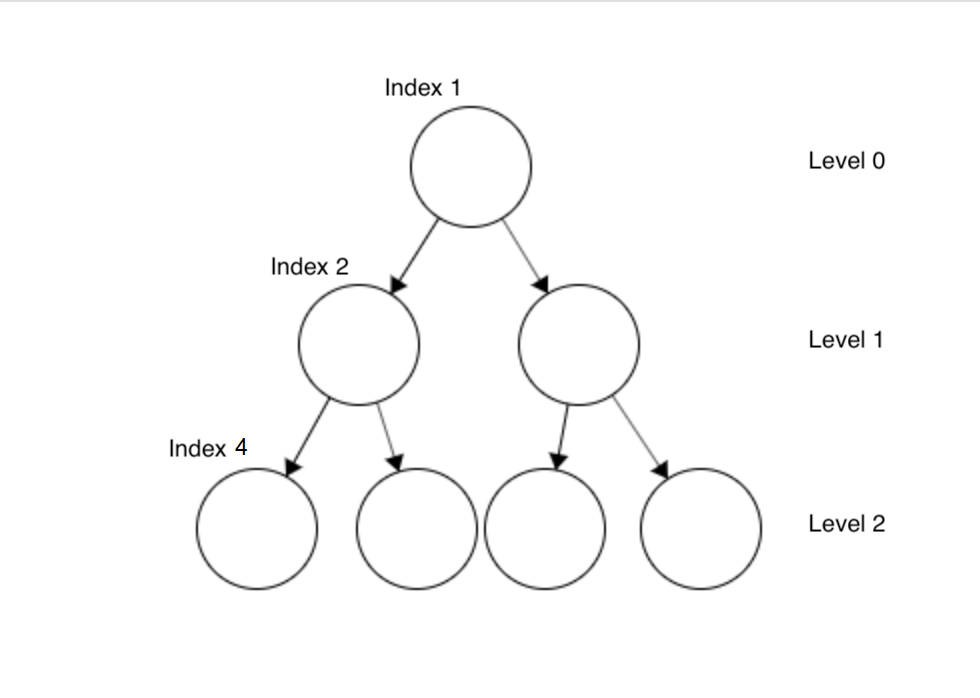
\includegraphics[width=10cm]{PSet2.png}
    \caption{A binary heap}
    \label{fig:heap}
\end{figure}

\item $P (x < a_j) = 1 - P(a_j \leq x) = 1 - p^j$. So the probability of $P(x < a_j) = 1 - p^j$.

\item $P(x < a_j \cap x < a_j_+_1) = 1 - p^j$. We note that the probability here is the same as in part c because $a_j \leq a_j_+_1$ as this is a binary min-heap. So if $x < a_j$ occurs then $x < a_j_+_1$ will also occur. So, $P(x < a_j \cap x < a_j_+_1)$ is dependent on $P (x < a_j)$. Thus $P(x < a_j \cap x < a_j_+_1) = 1 - p^j$.

\item $P(x < a_j_+_1 | x < a_j) = 1$. For conditional probability we are given $P(A|B) = \dfrac{P(A \cap B)}{P(B)}$. Here $P(A|B)$ is $P(x < a_j_+_1 | x < a_j)$, $P(A \cap B)$ is $P(x < a_j_+_1 \cap x < a_j)$, and $P(B)$ is $P(x < a_j)$. So, $P(x < a_j_+_1 | x < a_j) = \dfrac{P(x < a_j \cap x < a_j_+_1)}{P (x < a_j)} = \dfrac{1-p^j}{1 - p^j} = 1$.

\item $P(x < a_j | x < a_j_+_1) = \dfrac{1-p^j}{1 - p^j^+^1}$. For conditional probability we are given $P(A|B) = \dfrac{P(A \cap B)}{P(B)}$. Here $P(A|B)$ is $P(x < a_j | x < a_j_+_1)$, $P(A \cap B)$ is $P(x < a_j \cap x < a_j_+_1)$, and $P(B)$ is $P (x < a_j_+_1)$. $P(x < a_j_+_1) = 1 - P(a_j_+_1 \leq x) = 1 - p^j^+^1$. So, $P(x < a_j | x < a_j_+_1) = \dfrac{P(x < a_j \cap x < a_j_+_1)}{P(x < a_j_+_1)} = \dfrac{1-p^j}{1 - p^j^+^1}$.


\item $P(a_j \leq x | x < a_j_+_1) = \dfrac{p^j - p^j^+^1}{1 - p^j^+^1}$. For conditional probability we are given $P(A|B) = \dfrac{P(A \cap B)}{P(B)}$. Here $P(B)$ is $P(x < a_j_+_1) = 1 - p^j^+^1$. $P(A \cap B)$ is $P(a_j \leq x \cap x < a_j_+_1) = 1 - P(x < a_j) - P(a_j_+_1 \leq x) = 1 - (1 - p^j) - p^j^+^1 = p^j - p^j^+^1$. Note that we are looking for the probability of $a_j \leq x < a_j_+_1$, so to find this, we simply subtract from 1 the probability of $x < a_j$ and $a_j_+_1 \leq x$ so that we are left with just the probability of the intersection. So,  $P(a_j \leq x | x < a_j_+_1) = \dfrac{P(a_j \leq x \cap x < a_j_+_1)}{P(x < a_j_+_1)} = \dfrac{p^j - p^j^+^1}{1 - p^j^+^1}$.  

\item
Q.insert(x) would only perform one swap if $x$ is less than its parent but not less than its parent's parent. In other words if $x$ was inserted at the bottom of the tree say at index $a_k_+_1$ then for only one swap to occur, $a_k$ should be greater than $x$ and $a_k_-_1$ should be less than or equal to x.

\item The probability that Q.insert(x) performs exactly one swap based on the condition given in part $h.)$ is given by $p^k^-^1 - p^k$. This is because the probability of only swap occurring is given by $P(a_k_-_1 \leq x \cap x < a_k) = 1 - P(x < a_k_-_1) - P(a_k \leq x) = 1 - (1 - p^k^-^1) - p^k = p^k^-^1 - p^k$.

\item
Q.insert(x) would only perform two swap if $x$ is less than its parent and less than its parent's parent but greater than its parent's parents parent. In other words if $x$ was inserted at the bottom of the tree say at index $a_k_+_1$ then for the first swap to occur, $a_k$ should be greater than $x$. For the second swap to occur then $x$ should be less than $a_k_-_1$ and it's other child but for another not to occur x should not be less than $a_k_-_2$. 

\item The probability of Q.insert(x) performing two swaps based on the condition given in part $j.)$ is given by $p^k^-^2 - p^k^-^1$. This is because the probability of only two swaps occurring is given by $P(a_k_-_2 \leq x \cap x < a_k_-_1) = 1 - P(x < a_k_-_2) - P(a_k_-_1 \leq x) = 1 - (1 - p^k^-^2) - p^k^-^1 = p^k^-^2 - p^k^-^1$.

\item Q.insert(x) would perform  exactly $j$ swaps when $x$ is less than $j$ of its parents. That is to say, $x$'s parent's parent's ... parent $j$ times. To simplify this, let's denote $x$'s parent with $parent_1$ and $x$'s parent's parent with $parent_2$ and so on till we reach $parent_j$. If $x < parent_j_+_1$, then we would have performed $j+1$ swaps assuming that $x$ is inserted at position $a_k_+_1$. So to ensure that only $j$ swaps are performed we require $x < a_k_-_j_+_1$ and $x \geq a_k_-_j$.  

\item The probability of Q.insert(x) performing $j$ swaps based on the condition given in part $l.)$ is given by $p^k^-^j - p^k^-^j^+^1$. This is because the probability of only $j$ swaps occurring is given by $P(a_k_-_j \leq x \cap x < a_k_-_j_+_1) = 1 - P(x < a_k_-_j) - P(a_k_-_j_+_1 \leq x) = 1 - (1 - p^k^-^j) - p^k^-^j^+^1 = p^k^-^j - p^k^-^j^+^1$. 

\item The expected number of swaps for Q.insert(x) is $E(m) = \sum_{j=0}^{m} j \cdot (p^{k-j} -p^{k-j+1})$. This is because the expected value of $Y$ is the summation of $y_i$ multiplied by $p(y_i)$, where $p(y_i)$ is the probability of event $y_i$ occurring, and $y_i$ for $i = 1,..,n$, is the number of finite outcomes. 

\end{enumerate}

\end{document}
